\documentclass[12pt]{book}

\usepackage{tikz}
\usetikzlibrary{patterns}
\usepackage{graphicx}
\usepackage{caption}
\usepackage{svg}

\usepackage{csquotes}
\usepackage{esdiff}
\usepackage{amsmath}
\usepackage{amsthm}
\usepackage{mathrsfs}
\usepackage{siunitx}
\usepackage{amsthm}

\newcounter{myremark}[chapter]
\renewcommand{\themyremark}{Remark \thechapter.\arabic{myremark}}
\makeatletter
\newenvironment{remark}[1][]{
    \refstepcounter{myremark}
    \noindent\ignorespaces
    \begin{description}
        \item[\themyremark\space\ifx\relax#1\relax\else(#1) \fi:]
            }{
    \end{description}%
}
\makeatother


\newtheoremstyle{bfnote}
{}{}
{\itshape}{}
{\bfseries}{.}
{ }{\thmname{#1}\thmnumber{ #2}\thmnote{ (#3)}}
\theoremstyle{bfnote}

% \theoremstyle{bfnote}
% \newtheorem{definition}{Definition}[chapter]

% \theoremstyle{bfnote}
% \newtheorem{axiom}{Axiom}[chapter]

% \theoremstyle{bfnote}
% \newtheorem{law}{Law}[chapter]

% \theoremstyle{bfnote}
% \newtheorem{lemma}{Lemma}[chapter]

% \theoremstyle{bfnote}
% \newtheorem{proposition}{Proposition}[chapter]

% \theoremstyle{bfnote}
% \newtheorem{theorem}{Theorem}[chapter]

% \theoremstyle{bfnote}
% \newtheorem{collorary}{Corollary}[Theorem]

% \theoremstyle{bfnote}
% \newtheorem{principle}{Principle}[chapter]

\theoremstyle{bfnote}
\newtheorem{problem}{Problem}[chapter]


\usepackage[ a4paper, margin = 1 in ]{geometry}

\DeclareSIUnit{\RPM}{RPM}

\begin{document}

\chapter{Formulation of the Problem} % (fold)
\label{chap:Formulation_of_the_Problem}

We will compute the flow field of the airflow within the inlet of the engine. To this end, a full-computation of the domain by Navier-Stokes equation is the supreme approach. However, computation of the whole Navier-Stokes equation without any approximation seems computationally costs as problem does not pose any unstable effect. We will justify this fact later. However, we propose a geometrical prototype for the flow field is as follow:

\begin{problem}
    Consider a cylinder of radius $R_2$ and the length $H_2$. Inside the cylinder, there is a cone of radius $R_1$ and height $H_1$ (half angle $\psi$). This cone is at the end of cylinder. The flow through the cylinder have the undisturbed velocity of $U_{\infty}$ at the beginning of the inlet. The cone rotates at the angular velocity $\omega$, which induces swirl component for flow field.
\end{problem}

At the cruise condition, the air has the following properties:
\[
\begin{array}{lcl}
    h & \cdots\cdots\cdots & \SI{10000}{\meter} \\
    \rho_\infty & \cdots\cdots\cdots & \SI{0.38671}{\kilogram\cubic\meter} \\
    T_\infty & \cdots\cdots\cdots & \SI{238.15}{\kelvin} \\
    p_\infty & \cdots\cdots\cdots & \SI{26436}{\pascal} \\
    c & \cdots\cdots\cdots & \SI{309.36}{\meter\per\second} \\
    \mu & \cdots\cdots\cdots & \SI{0.00001552}{\pascal\second} \\
\end{array}
\]
where we use the ISA condition with the sea level offset temperature $T = \SI{15}{\degreeCelsius}$ to calculate the above table.

As at the cruise condition, we do not take into account the effect of the ground vortices. All the secondary effect such as the vibration of the nacelle inlet and the cone, as well as all the roughness of the surface will be neglected. Furthermore, as the Mach number of the free stream flow is about $0.85$, which is the cruise speed of the airplane, there is no reason to ignore the compressibility of the flow at first glance. However, we will neglect it as the flow profile of entrance air does not change dramatiscally in term of temperature, pressure and density. It arrives at the first approximation that the flow field is incompressible.

Now we estimate qualitatively the effect of viscosity in the first flow. To this end, Reynold number around the cone is computed:
\begin{align}
    \mathrm{Re} \approx \dfrac{\rho_{\infty} \Omega R_1}{\mu_{\infty}} = \dfrac{\SI{0.38671}{\kilogram\cubic\meter} \times \SI{319}{\radian\per\second} \times \SI{0.25}{\meter}}{\SI{0.00001552}{\pascal\second}} \approx 2 \times 10^6.
\end{align}
This calculation arrives from the fact that:
\begin{enumerate}
    \item The cone (spinner) is directly tied to the low-pressure (LP) shaft, which operates in the range of approximately $\SI{3000}{\RPM}$ to $\SI{5000}{\RPM}$ at cruise speed.
    \begin{align*}
        \Omega \approx \dfrac{\SI{4000}{\RPM} \times 2 \pi}{\SI{60}{\sec\per\min}} \approx \SI{420}{\radian\per\second}.
    \end{align*}
    \item The spinner base radius corresponds to the hub radius of the fan, which is dictated by the hub-to-tip ratio. For a typical modern turbofan engine, this ratio ranges from $0.2$ to $0.35$. For a turbofan engine with fan diameter $\SI{2}{\meter}$. Therefore
    \begin{align*}
        R_1 \approx 0.25 \times \SI{1}{\meter} = \SI{0.25}{\meter}
    \end{align*}
\end{enumerate}

This Reynold number is very large, which forces us to calculate the flow field using the model of \enquote{Very Large Reynold Number}. Indeed, the flow field is divided into two regions: the bulk region, where viscous effects are negligible, and the boundary-layer region, where all significant viscous effects are concentrated. In the boundary-layer, we will calculate all the viscosity-driven effects using perturbations from the inviscid solution. The same conclusion could be draw for the flow near the wall of the engine inlet (nacelle). In fact, the Reynolds number of the wall is
\begin{align*}
    Re \approx \dfrac{\rho_\infty U_{\text{wall}} R_2}{\mu_\infty} = \dfrac{\SI{0.38671}{\kilogram\cubic\meter} \times \SI{250.75}{\meter\per\second} \times \SI{0.5}{\meter}}{\SI{0.00001552}{\pascal\second}} \approx 3 \times 10^6.
\end{align*}
This calculation comes from the fact that the flow field at the cruise condition has the speed $U_{\text{wall}} \approx \SI{250.75}{\meter\per\second}$ for Mach 0.85 and the radius of the engine inlet is approximated about $\SI{0.5}{\meter}$.

Follow the model of \enquote{Very Large Reynold Number}, we proceed further by:
\begin{enumerate}
    \item assuming that the flow is inviscid and find an inviscid solution for the entire flow field.
    \item considering the boundary-layer as a small perturbation from the inviscid solution and try to solve them to get the pressure and friction profile along the cone surface.
\end{enumerate}

The first sub problem is important for the integration of motion equation of the detached ice and the second one is crucial for our analysis of the process of detachment itself.
% chapter Formulation of the Problem (end)

\section{Inviscid Solution} % (fold)
\label{sec:Inviscid_Solution}
Although the cone has a non-null rotational speed $\Omega$, the flow field is fully potential since the flow is inviscid and therefore cannot induce any kind of rotation from the cone. This implies that the flow field is potential:
\begin{align}
    \Delta \phi(x, y, z) = 0.
\end{align}
Based on the axisymmetry of the domain, we could employ the cylindrical coordinate $r, \theta, z$ with $z$ is the axis of the cylinder oriented from the inlet to the oulet. If their is no deflection in inlet velocity direction $\underline{U}_\infty = U_\infty \underline{e}_z$ for constant $U_\infty$, then the variable $\theta$ does not enter the problem and we could write:
\begin{align}
    \Delta \phi(r, z) = 0.
\end{align}

The boundary condition for this potential flow is that on the cone surface and on the wall, its normal velocities should be vanished:
\begin{align}
    & \diffp{\phi}{r}(r = R_2) = 0\\
    & {\nabla \phi} \cdot \underline{n}_{\text{cone}} = 0.
\end{align}
At the entrance of the inlet, the velocity need to be uniform:
\begin{align}
    \dfrac{1}{r} \diffp{\phi}{r}(z = H_1 - H_2) & = U_\infty \\
    - \dfrac{1}{r} \diffp{\phi}{z}(z = H_1 - H_2) & = 0
\end{align}
This assumption is based on the fact that a uniform flow does not intefere engine performance. We will return to the problem of non-uniformity later.

At the exit of the inlet, we could assume the flow is uniform as the cone, at engineering intention, is used for correcting the air flow and make sure the uniformity of the entrance flow before entering the bypass fan or compressor. The reason is again to ensure the desired engine performance. Therefore, we could write:
\begin{align}
    & \diffp{\phi}{z}(z = H_1) = U_2 \\
    & \diffp{\phi}{r}(z = H_1) = 0
\end{align}
But this assumption is not physcially possible as it serves as a flow diflection rather than the flow correction role of the spinner. So that we will extend the inlet wall to length $H_3$ and extend the base of the cone with a cylinder of height $H_3$, to channel the flow. This imaginable domain does not contribute to the final solution but it helps us simulate the flow more naturally. Therefore, we just extract the physical domain. There is no strict constraint for the dimension $H_3$, but we will conduct several case studies to find the optimal value of $H_3$ so that the solution is not computationally expensive and reserved the precision. We represent the new domain as follow:
\begin{figure}[h!]
    \centering
    \begin{tikzpicture}
        \draw[fill=blue!20, draw=black, thick] (0,0) -- (3,0) -- (6,2) -- (9,2) -- (9,4) -- (0,4) -- (0,0) -- cycle;
        \draw[dashed] (3,0) -- (9,0) ;
        \draw[dashed] (9,0) -- (9,2) ;
        \draw[dashed] (6,2) -- (6,4) ;
        \fill[pattern=north east lines] (6,2) rectangle (9,4);
        \node[below] at (4.5,1) {$\mathscr{B}_1$};
        \node[below] at (9.5,3) {$\mathscr{B}_2$};
        \node[below] at (-0.5,2) {$\mathscr{B}_3$};
        \node[below] at (4.5,4.8) {$\mathscr{B}_4$};
        \node[below] at (6.75,1) {spinner};
    \end{tikzpicture}
    \caption{The model of the engine inlet with the hatched region is the imaginable domain. The figure represents only the cutting face $\theta = 0$ due to axisymmetry.}
    \label{fig:simplified_flow_dom}
\end{figure}

\subsection{Laplace Equation with Diriclet Boundary Condition for Streamline Function} % (fold)
\label{subsec:Laplace_Equation_with_Diriclet_Boundary_Condition_for_Streamline_Function}

As discussed earlier, the inviscid solution is formulated by streamline function. The streamline function is constant along each streamline, this gives us a mean to solve the problem by the Laplace equation with Diriclet condition:
\begin{align}
    \Delta \psi(r, z) = 0,
\end{align}
where the velocitie is calculated as follows:
\begin{align}
    u_z = \dfrac{1}{r} \diffp{\phi}{r}(r,z) \quad \text{and} \quad u_r = - \dfrac{1}{r} \diffp{\phi}{r}(r, z).
\end{align}

We represent the flow domain by the following figure (Fig~\ref{fig:simplified_flow_dom}) where we add an imagined domain to make the flow:
\begin{enumerate}
    \item The edge $\mathscr{B}_1$ represent the axis $z$ from $z = H_1 - H_2$ to the vertex of the cone $z = 0$, plus the surface of the spinner, plus the surface $r = R_1$ from $z = H_1$ to $H_3$. $\mathscr{B}_1$ is a streamline.
    \item The edge $\mathscr{B}_2$ represents the exit of the inlet.
    \item The edge $\mathscr{B}_3$ represents the entrance of the engine inlet.
    \item The edge $\mathscr{B}_4$ represents the wall of the inlet.
\end{enumerate}

From this domain name convention, we could write directly the boundary condition for the streamline function:
\begin{align}
    \left. \psi \right|_{\mathscr{B}_1} = 0, \quad \left. \psi \right|_{\mathscr{B}_2} = \dfrac{1}{2} U_2 \left( r^2 - R_1^2 \right), \quad \left. \psi \right|_{\mathscr{B}_3} = \dfrac{1}{2} U_1 R_1^2, \quad \left. \psi \right|_{\mathscr{B}_4} = \dfrac{1}{2} U_1 r^2
\end{align}
The condition in $\mathscr{B}_1$ and $\mathscr{B}_4$ is due to the fact that $\psi$ is constant along the streamline. The absolute value of them are not important as long as their difference $\left. \psi \right|_{\mathscr{B}_4} - \left. \psi \right|_{\mathscr{B}_1} = U_1 R_2^2/2$ is the volume flow rate. So, we choose $\left. \psi \right|_{\mathscr{B}_1} = 0$ to simplify the calculation. The velocity $U_2$ at the exit is calculated by the by the mass conservation as follow:
\begin{align}
    U_2 = U_1 \dfrac{R_1^2}{R_1^2 - R_2^2}
\end{align}
% subsection Laplace Equation with Diriclet Boundary Condition for Streamline Function (end)

\subsection{Finite Element Method Solution} % (fold)
\label{subsec:Finite_Element_Method_Solution}
Due to the axisymmetric essence of the flow field, we would like to apply the axisymmetric element. This choice will reduce enormously the computational cost instead of a full-tridimensional model. The philosophy is to convert the tridimensional ring element to a two-dimensional element. For this end, we represent the grid for the cutting face $\theta = 0$.

\begin{figure}[h!]
    \centering
    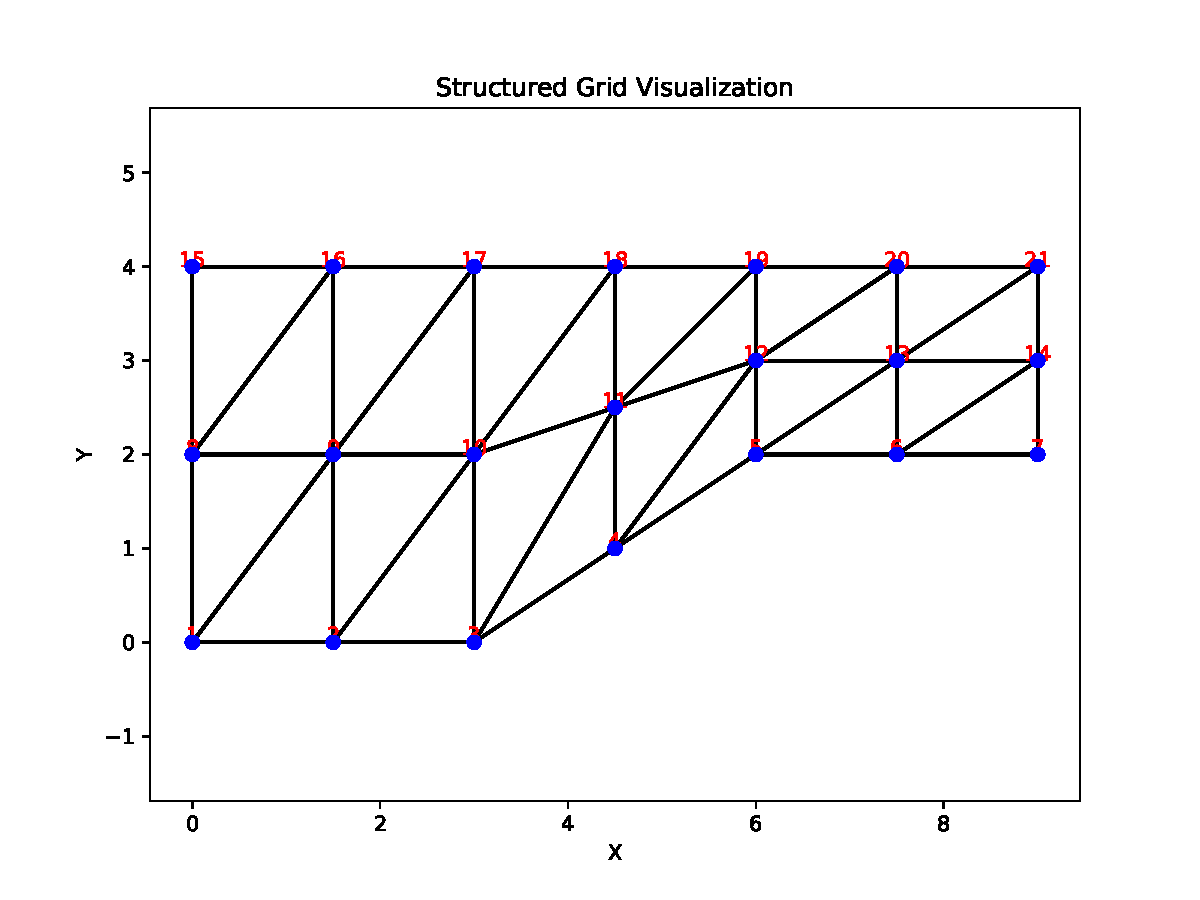
\includegraphics[width=0.8\textwidth, height=0.6\textheight, keepaspectratio]{triangular_grid.pdf}
    \caption{A structured grid with node numbering available.}
    \label{fig:structured_grid}
\end{figure}

We choose this element as they are all triangular which provides more flexibility. The nodes coordinates are calculated for three domains as follows:
\begin{enumerate}
    \item For the first rectangular domain:
    \begin{align}
        x[i][j] = \dfrac{H_1}{M_1}(i - 1), \quad y[i][j] = \dfrac{L_1}{N}(j - 1)
    \end{align}
    \item For the squared trapezoid domain:
    \begin{equation}
        \begin{aligned}
            & x[i][j] = H_1 + \dfrac{H_2}{M_1}(i - M_1 - 1), \\
            & y[i][j] = \dfrac{R_1}{H_2} \left( 1 - \dfrac{j - 1}{N} \right) x[i][j] + \dfrac{R_1}{N}(j - 1) - \dfrac{R_1}{H_1} H_2 \left( 1 - \dfrac{j - 1}{N} \right) \\
        \end{aligned}
    \end{equation}
    \item For the second rectangular domain:
    \begin{align}
        x[i][j] = H_1 + H_2 + \dfrac{H_3}{M_3}(i - M_1 - M_2 - 1), \quad y[i][j] = \dfrac{L_1}{N}j
    \end{align}
\end{enumerate}
where $M_1$, $M_2$, and $M_3$ stand for the number of elements in the horizontal direction and $N$ is the number of elements in the vertical direction. The total number of isoparametric unilateral elements in the domain is therefore $N \times (M_1 + M_2 + M_3)$, and the number of rectangle elements is double the total number of the former.

We choose this kind of discretization as all node with constant $j$ will lies near the streamline of the flow field. The algorithm to solve the finite element method follows the conventional algorithm with the local stiffness matrix. After the solution, we obtain the value of $\psi$ at each node. However, this raw value of $\psi$ can not be used to calculate the velocity as it lack of continuity. In fact, we choose the $C^0$ element to save the computational effort. This means that if we use the interpolation to reconstruct the gradient of $\psi$, the obtained gradient will be definitely piece-wise continuous with the strict discoutinuous across element. This result is non sense as long as we calculate the gradient of $\psi$ across boundary of elements or at nodes. Therefore, in the next subsection, we will discuss a method to reconstruct the gradient of $\psi$ with the continuity across all element.
% subsection Finite Element Method Solution (end)

\subsection{Post-Processing for Gradient of Streamline Function} % (fold)
\label{subsec:Post-Processing_for_Gradient_of_Streamline_Function}
The method to reconstruct the gradient of the streamline function emerged from the earliest day of FEM. There are plenty of litterature source discuss about this subject. Amongst them, Recovery by Equilibration of Patches (REP), Superconvergent Patch Recovery (SPR) are the most popular one. However, we will employ a new gradient recovery method [need citation here]. This method has the advantage of ease to implement.

For the raw derivative, the interpolation function is a polynomial of degree $1$, which causes the discoutinuity across the edges of each element. Therefore, our purpose is to construct a polynomial of degree at least $2$ to approximate the gradient of $\psi$. In our case, we should only compute a polynomial of degree $2$ which has the form:

\begin{align}
    P_2(x,y) = a_1 + a_2 x + a_3 y + a_4 x^2 + a_5 xy + a_6 y^2.
\end{align}
We will find this polynomial by fitting in the sense of least square. For that end, we select all nodes that is connected to $v_i$ as the patch of $v_i$. As the form of $P_2(x,y)$, we need at least 6 other nodes connects to $v_i$. For a vertex $v_i$, let $\ell_i$ be the length of the longest edge attached to $v_i$. 

Suppose that the number of node is sufficient, namely, $v_{i1}$, $v_{i2}$, $\ldots$, $v_{in}$. Using the local coordinate system $(\xi, \eta)$ with the origin at $v_i$ for each point $v_{ij}$:
\begin{align}
    (\xi_j, \eta_j) = \dfrac{(x_{ij},y_{ij}) - (x_i,y_i)}{\ell_i}
\end{align}

The coefficient $\hat{a} := (a_1, \ldots, a_6)^T$ of the fitting polynomial is computed from the equation:
\begin{align}
    A^T A \hat{a} = A^T B,
\end{align}
where
\begin{align*}
    A = \begin{pmatrix}
        1 & \xi_1 & \eta_1 & \cdots & \eta_1^{k+1} \\
        1 & \xi_2 & \eta_2 & \cdots & \eta_2^{k+1} \\
        1 & \xi_3 & \eta_3 & \cdots & \eta_3^{k+1} \\
        \vdots & \vdots & \vdots & \ddots & \vdots \\
        1 & \xi_n & \eta_n & \cdots & \eta_n^{k+1}
    \end{pmatrix},
    \quad \text{and} \quad
    B = \begin{pmatrix}
        \psi(v_{i1}) \\
        \psi(v_{i2}) \\
        \vdots \\
        \psi(v_{in})
    \end{pmatrix}
\end{align*}
With the result of $\hat{a}$, we could calculate the derivative of $\psi$ at the node $v_i$:
\begin{align*}
    \dfrac{\partial \psi}{\partial x} (v_i) = \dfrac{a_2}{\ell_i}, \quad \dfrac{\partial \psi}{\partial y} (v_i) = \dfrac{a_3}{\ell_i}
\end{align*}

\begin{align*}
    \dfrac{\partial^2 \psi}{\partial x^2} (v_i) = 2\dfrac{a_4}{\ell_i^2}, \quad \dfrac{\partial^2 \psi}{\partial x \partial y} (v_i) = \dfrac{a_5}{\ell_i^2}, \quad \text{and} \quad \dfrac{\partial^2 \psi}{\partial y^2} (v_i) = 2\dfrac{a_6}{\ell_i^2}
\end{align*}

From this recovery gradient each vertex, we are able to compute the recovered gradient field by interpolation using the finite element basis functions.

If a node located on the boundary has fewer connected nodes: two, three, or four nodes typically. To ensure that there are enough nodes for constructing the polynomial, we include:
\begin{enumerate}
    \item All the nodes that are directly connected to the boundary node to form an original node.
    \item And all the nodes that are connected to the internal nodes in the original patch. This will include all the nodes needed.
\end{enumerate}

\begin{remark}
    For the general case of polynomial of order $k$, the number of points needed is at least
    \begin{align*}
        n = \dfrac{(k + 1)(k + 2)}{2}
    \end{align*}

    In the case of a node does not connect to at least, namely five nodes at maximum. We proceed by the same manner, and instead of searching for all the node in the radius $\ell_i$ to $v_i$, we search for all nodes in the radius $2\ell_i$.
\end{remark}

% subsection Post-Processing for Gradient of Streamline Function (end)











% \begin{align*}
%     \phi(r, z) = U_{\infty} z + A \left( e^{-kz} - \dfrac{e^{kz}}{e^{-2k(H_1 - H_2)}} \right) \left[ J_0(kr) - \dfrac{J_0'(kR_2)}{Y_0'(kR_2)}Y_0(kr) \right]
% \end{align*}

% Where $k$ is solved by the equation:

% \begin{align*}
%     & k A \left( e^{-kz} - \dfrac{e^{kz}}{e^{-2k(H_1 - H_2)}} \right) \left[ J_0'(k\tan\psi z) - \dfrac{J_0'(kR_2)}{Y_0'(kR_2)}Y_0'(k\tan\psi z) \right] = \\
%     & \left[ U_{\infty} + k A\left( e^{-kz} - \dfrac{e^{kz}}{e^{-2k(H_1 - H_2)}} \right) \left(J_0 (k\tan\psi z) - \dfrac{J_0'(kR_2)}{Y_0'(kR_2) Y_0(k\tan\psi z)} \right)\right]\tan\psi
% \end{align*}

% We can use Newton method to solve for $k$.




% \begin{align*}
%     \phi(r, z) = U_{\infty} z + A \cos(kz) J_0(-kr)
% \end{align*}






% The effect of the spinning cone is modeled as some vortices sheets or lines.




% section Inviscid Solution (end)


% \section{Boundary-Layer on the Wall} % (fold)
% \label{sec:Boundary_Layer_on_the_Wall}

% It is just the pipe flow. 

% % section Boundary-Layer on the Wall (end)


% \section{Boundary-Layer on the Cone} % (fold)
% \label{sec:Boundary_Layer_on_the_Cone}

% Axisymmetric boundary layers
% \begin{align*}
%     & \diffp{(r_w \rho u)}{x} + \diffp{(r_w \rho v)}{x} = 0 \\
%     & \rho \left( u\diffp{u}{x} + thev\diffp{v}{x} - \dfrac{w^2}{r_w}\diff{r_w}{x} \right) = -\diffp{p}{x} + \diffp{}{y}\left(\mu\diffp{u}{y}\right) \\
%     & \rho \left( u\diffp{w}{x} + v\diffp{w}{y} + \dfrac{uw}{r_w} \diff{r_w}{x} \right) = \diffp{}{y}\left( \mu \diffp{w}{y} \right) \\
%     & \rho c_p \left(u\diffp{T}{x} + v\diffp{T}{y}\right) = \diffp{}{y}\left(\lambda \diffp{T}{y}\right) + \beta T u \diff{p}{x} + \mu\left[\left(\diffp{u}{y}\right)^2 + \left(\diffp{v}{y}\right)^2\right]
% \end{align*}

% In our case $r_w (x) = x \tan\psi$. The component of the wall shear stress are
% \begin{align*}
%     \tau_{wx} = \mu \left( \diffp{u}{y} \right)_w \quad 
%     \tau_{wz} = \mu \left( \diffp{w}{y} \right)_w
% \end{align*}

% The displacement and momentum thickness

% section Boundary-Layer on the Cone (end)




\end{document}